\section{角动量算符}

\begin{quotation}
``只要一门科学分支能提出大量的问题,它就充满着生命力,而问题缺乏则预示着独立发展的衰亡和终止。''\qquad 希尔伯特
\end{quotation}

\subsection{角动量算符}

经典力学中角动量的定义是:

\begin{equation}\label{classical angular momentum}
\vec L = \vec r \times \vec p
\end{equation}

$\vec L$可用来描述地球围绕太阳的运动,也叫轨道角动量(Orbital angular momentum)\index{Orbital angular momentum: 轨道角动量},以区别于后面我们将要讨论的自旋角动量(Spin angular momentum)。在经典力学中自旋角动量与轨道角动量相比没有本质的区别,因为地球的自转(或更广义地说是刚体的自转)可看做是一系列距离自转轴心远近不同的质量微元($dm$)做“轨道运动”的叠加。

\index{Angular momentum: 角动量}

在直角坐标系($x, y, z$)下,角动量算符($\hat L$)可表示为:

\begin{equation}
\left\{ \begin{array}{l}
 \widehat L_x  = y\widehat p_z  - z\widehat p_y  = \frac{\hbar }{i}\left( {y\frac{\partial }{{\partial z}} - z\frac{\partial }{{\partial y}}} \right) \\
 \widehat L_y  = z\widehat p_x  - x\widehat p_z  = \frac{\hbar }{i}\left( {z\frac{\partial }{{\partial x}} - x\frac{\partial }{{\partial z}}} \right) \\
 \widehat L_z  = x\widehat p_y  - y\widehat p_x  = \frac{\hbar }{i}\left( {x\frac{\partial }{{\partial y}} - y\frac{\partial }{{\partial x}}} \right) \\
 \end{array} \right.
\end{equation}

角动量算符的平方($\hat L^2$)被定义为:

\begin{equation}
\hat L^2 =\hat L \cdot \hat L = L_x^2 + L_y^2 + L_z^2 
\end{equation}

展开为:

\begin{equation}
\widehat L^2  =  - \hbar ^2 \left[ {\left( {y\frac{\partial }{{\partial z}} - z\frac{\partial }{{\partial y}}} \right)^2  + \left( {z\frac{\partial }{{\partial x}} - x\frac{\partial }{{\partial z}}} \right)^2  + \left( {x\frac{\partial }{{\partial y}} - y\frac{\partial }{{\partial x}}} \right)^2 } \right]
\end{equation}


现在,设法变到球坐标$\left( {r,\theta ,\varphi } \right)$下:


\begin{figure}[h]
\begin{center}
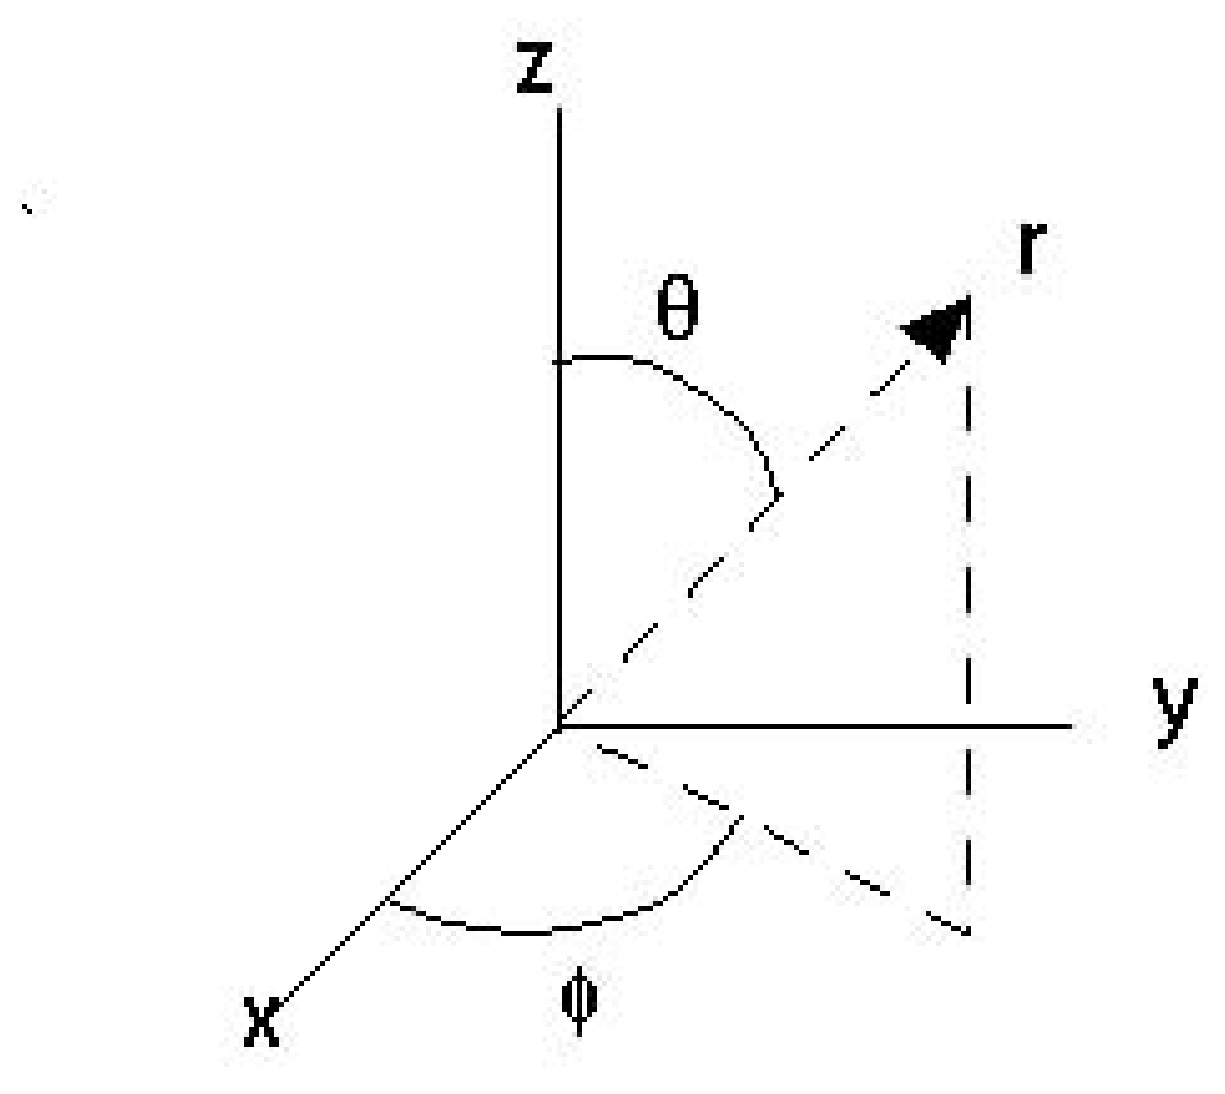
\includegraphics[clip,width=6cm]{AngularMomentum/14-1.ps}
\caption{球坐标示意图}
\end{center}
\end{figure}

\begin{equation}
\left\{ \begin{array}{l}
 x = r\sin \theta \cos \varphi  \\
 y = r\sin \theta \sin \varphi  \\
 z = r\cos \theta  \\
 r^2  = x^2  + y^2  + z^2  \\
 \cos \theta  = {\textstyle{z \over r}} \\
 \tan \varphi  = {\textstyle{y \over x}} \\
 \end{array} \right.
\end{equation} 
 
我们需要求出$\frac{\partial r}{\partial x}$, $\frac{\partial r}{\partial y}$和$\frac{\partial r}{\partial z}$:
 
\begin{equation}
\left\{ \begin{array}{l}
 \frac{{\partial r}}{{\partial x}} = \frac{\partial }{{\partial x}}\left( {x^2  + y^2  + z^2 } \right)^{{\textstyle{1 \over 2}}}  = \frac{x}{r} = \sin \theta \cos \varphi  \\
 \frac{{\partial r}}{{\partial y}} = \frac{\partial }{{\partial y}}\left( {x^2  + y^2  + z^2 } \right)^{{\textstyle{1 \over 2}}}  = \frac{y}{r} = \sin \theta \sin \varphi  \\
 \frac{{\partial r}}{{\partial z}} = \frac{\partial }{{\partial z}}\left( {x^2  + y^2  + z^2 } \right)^{{\textstyle{1 \over 2}}}  = \frac{z}{r} = \cos \theta  \\
\end{array} \right.
\end{equation}

还有$\frac{\partial \theta}{\partial x}$,$\frac{\partial \theta}{\partial y}$和$\frac{\partial \theta}{\partial z}$: 
 
 $\cos \theta  = \frac{z}{r}$,两边对x求导:$ - \sin \theta \frac{{\partial \theta }}{{\partial x}} = \frac{{ - z}}{{r^2 }}\frac{{\partial r}}{{\partial x}}$,

\begin{equation}
\frac{{\partial \theta }}{{\partial x}} = \frac{1}{{\sin \theta }}\frac{z}{{r^2 }}\frac{{\partial r}}{{\partial x}} = \frac{1}{{\sin \theta }}\frac{{r\cos \theta }}{{r^2 }}\sin \theta \cos \varphi  = \frac{1}{r}\cos \theta \cos \varphi
\end{equation}

$\cos \theta  = \frac{z}{r}$,两边对y求导:$ - \sin \theta \frac{{\partial \theta }}{{\partial y}} = \frac{{ - z}}{{r^2 }}\frac{{\partial r}}{{\partial y}}$

\begin{equation}
\frac{{\partial \theta }}{{\partial y}} = \frac{1}{{\sin \theta }}\frac{z}{{r^2 }}\frac{{\partial r}}{{\partial y}} = \frac{1}{{\sin \theta }}\frac{{\cos \theta }}{r}\sin \theta \sin \varphi  = \frac{1}{r}\cos \theta \sin \varphi
\end{equation}

$\cos \theta  = \frac{z}{r}$,两边对z求导:$ - \sin \theta \frac{{\partial \theta }}{{\partial z}} = \frac{{r - z{\textstyle{{\partial r} \over {\partial z}}}}}{{r^2 }} = \frac{1}{r} - \frac{z}{{r^2 }}\frac{{\partial r}}{{\partial z}}$

\begin{equation}
\frac{{\partial \theta }}{{\partial z}} =  - \frac{1}{{r\sin \theta }} + \frac{1}{{\sin \theta }}\frac{z}{{r^2 }}\frac{{\partial r}}{{\partial z}} =  - \frac{1}{{r\sin \theta }} + \frac{1}{{\sin \theta }}\frac{{\cos \theta }}{r}\cos \theta  = \frac{{ - \sin ^2 \theta }}{{r\sin \theta }} =  - \frac{{\sin \theta }}{r}
\end{equation}

最后还有$\frac{\partial \varphi}{\partial x}$,$\frac{\partial \varphi}{\partial y}$和$\frac{\partial \varphi}{\partial z}$:

$\tan \varphi  = \frac{y}{x}$, 两边对x求导:$\sec ^2 \varphi \frac{{\partial \varphi }}{{\partial x}} = \frac{{ - y}}{{x^2 }}$,

\begin{equation}
\frac{{\partial \varphi }}{{\partial x}} = \frac{{ - y}}{{\sec ^2 \varphi }}\frac{1}{{x^2 }} = \frac{{ - r\sin \theta \sin \varphi }}{{\sec ^2 \varphi r^2 \sin ^2 \theta \cos ^2 \varphi }} =  - \frac{{\sin \varphi }}{{r\sin \theta }}
\end{equation}

$\tan \varphi  = \frac{y}{x}$, 两边对y求导:$\sec ^2 \varphi \frac{{\partial \varphi }}{{\partial y}} = \frac{1}{x}$,

\begin{equation}
\frac{{\partial \varphi }}{{\partial y}} = \frac{1}{{x\sec ^2 \varphi }} = \frac{{\cos ^2 \varphi }}{{r\sin \theta \cos \varphi }} = \frac{{\cos \varphi }}{{r\sin \theta }}
\end{equation}

$\tan \varphi  = \frac{y}{x}$, 两边对z求导:$\sec ^2 \varphi \frac{{\partial \varphi }}{{\partial z}} = 0$, 

\begin{equation}
\frac{{\partial \varphi }}{{\partial z}} = 0
\end{equation}

因此:

\begin{center}
$\left\{ \begin{array}{l}
 \frac{\partial }{{\partial x}} = \frac{{\partial r}}{{\partial x}}\frac{\partial }{{\partial r}} + \frac{{\partial \theta }}{{\partial x}}\frac{\partial }{{\partial \theta }} + \frac{{\partial \varphi }}{{\partial x}}\frac{\partial }{{\partial \varphi }} = \sin \theta \cos \varphi \frac{\partial }{{\partial r}} + \frac{{\cos \theta \cos \varphi }}{r}\frac{\partial }{{\partial \theta }} - \frac{{\sin \varphi }}{{r\sin \theta }}\frac{\partial }{{\partial \varphi }} \\
 \frac{\partial }{{\partial y}} = \frac{{\partial r}}{{\partial y}}\frac{\partial }{{\partial r}} + \frac{{\partial \theta }}{{\partial y}}\frac{\partial }{{\partial \theta }} + \frac{{\partial \varphi }}{{\partial y}}\frac{\partial }{{\partial \varphi }} = \sin \theta \sin \varphi \frac{\partial }{{\partial r}} + \frac{{\cos \theta \sin \varphi }}{r}\frac{\partial }{{\partial \theta }} + \frac{{\cos \varphi }}{{r\sin \theta }}\frac{\partial }{{\partial \varphi }} \\
 \frac{\partial }{{\partial z}} = \frac{{\partial r}}{{\partial z}}\frac{\partial }{{\partial r}} + \frac{{\partial \theta }}{{\partial z}}\frac{\partial }{{\partial \theta }} + \frac{{\partial \varphi }}{{\partial z}}\frac{\partial }{{\partial \varphi }} = \cos \theta \frac{\partial }{{\partial r}} - \frac{{\sin \theta }}{r}\frac{\partial }{{\partial \theta }} \\
 \end{array} \right.$
\end{center}

所以:

\begin{center}
$\left\{ \begin{array}{l}
 \widehat L_x  = \frac{\hbar }{i}\left( {y\frac{\partial }{{\partial z}} - z\frac{\partial }{{\partial y}}} \right) = i\hbar \left( {\sin \varphi \frac{\partial }{{\partial \theta }} + \cot \theta \cos \varphi \frac{\partial }{{\partial \varphi }}} \right) \\
 \widehat L_y  = \frac{\hbar }{i}\left( {z\frac{\partial }{{\partial x}} - x\frac{\partial }{{\partial z}}} \right) = i\hbar \left( { - \cos \varphi \frac{\partial }{{\partial \theta }} + \cot \theta \sin \varphi \frac{\partial }{{\partial \varphi }}} \right) \\
 \widehat L_z  = \frac{\hbar }{i}\left( {x\frac{\partial }{{\partial y}} - y\frac{\partial }{{\partial x}}} \right) =  - i\hbar \frac{\partial }{{\partial \varphi }} \\
 \end{array} \right.$
\end{center}

代入总角动量的平方$\hat L^2 = L_x^2 + L_y^2 + L_z^2$,经过计算,得到:

\begin{equation}
\widehat L^2   =  - \hbar ^2 \left[ {\frac{1}{{\sin \theta }}\frac{\partial }{{\partial \theta }}\left( {\sin \theta \frac{\partial }{{\partial \theta }}} \right) + \frac{1}{{\sin ^2 \theta }}\frac{{\partial ^2 }}{{\partial \varphi ^2 }}} \right]
\end{equation}


球坐标下$\widehat L^2 ,\widehat L_z $可表示为:

\begin{equation}\label{14-1}
\left\{ \begin{array}{l}
 \widehat L^2  =  - \hbar ^2 \left[ {\frac{1}{{\sin \theta }}\frac{\partial }{{\partial \theta }}\left( {\sin \theta \frac{\partial }{{\partial \theta }}} \right) + \frac{1}{{\sin ^2 \theta }}\frac{{\partial ^2 }}{{\partial \varphi ^2 }}} \right] \\
 \widehat L_z  = \frac{\hbar }{i}\left( {x\frac{\partial }{{\partial y}} - y\frac{\partial }{{\partial x}}} \right) =  - i\hbar \frac{\partial }{{\partial \varphi }} \\
 \end{array} \right.
\end{equation}

由于$\left[ {\widehat L^2 ,\widehat L_z } \right] = 0$,$L^2$,$L_z$可共同取确定值,可求得$\left( {\widehat L^2 ,\widehat L_z } \right)$的共同本征态$\left| \lambda, \mu \right\rangle$,使:

\begin{eqnarray}
\hat L^2 \left| \lambda, \mu \right\rangle &  = & \lambda \left| \lambda, \mu \right\rangle \\
 L_z \left| \lambda, \mu \right\rangle & = & \mu \left| \lambda, \mu \right\rangle
\end{eqnarray}

同时成立。



\subsection{$\left( {\hat L^2 ,\hat L_z } \right)$的共同本征态}

\subsubsection{$\hat L _z$的本征值问题:}

\begin{equation}
\frac{\hbar }{i}\frac{\partial }{{\partial \varphi }}\Phi  = l_z \Phi 
\end{equation}

即:$\frac{{\Phi '}}{\Phi } = \frac{{il_z }}{\hbar }$, 求出:

\begin{equation}
\Phi  = C\exp \left( {\frac{{il_z \varphi }}{\hbar }} \right)
\end{equation}

周期性边条件:$\Phi \left( \varphi  \right) = \Phi \left( {\varphi  + 2\pi } \right)$, $\frac{{2\pi l_z }}{\hbar } = m2\pi $, $m = 0, \pm 1, \pm 2,...$, 即:

\begin{equation}
l_z  = m\hbar
\end{equation}

归一化:$\int_0^{2\pi } {\Phi ^* \Phi d\varphi }  = C^2 2\pi  = 1$, 得到:

\begin{equation}
C = \frac{1}{{\sqrt {2\pi } }}
\end{equation}

正交归一化本征函数:

\begin{equation}
\Phi _m (\varphi ) = \frac{1}{{\sqrt {2\pi } }}e^{im\varphi }
\end{equation}

即:$\widehat L_z \Phi _m (\varphi ) = m\hbar \Phi _m (\varphi )$;$m = 0, \pm 1, \pm 2,...$,叫磁量子数。


\subsubsection{$\hat L ^2$本征值问题}

$\hat L ^2$与$\theta, \varphi$都有关,本征函数表示为$Y(\theta ,\varphi )$;

$\hat L ^2$本征值方程:

\begin{equation}
\widehat L^2 Y(\theta ,\varphi ) = \lambda \hbar ^2 Y(\theta ,\varphi )
\end{equation}

分离变量:$Y(\theta ,\varphi ) = \Theta (\theta )\Phi _m (\varphi )$,并且要求$Y(\theta ,\varphi )$同时也是$\widehat L_z $的本征函数;

\begin{equation}\label{14-2}
\frac{1}{{\sin \theta }}\frac{d}{{d\theta }}\left( {\sin \theta \frac{{d\Theta }}{{d\theta }}} \right) + \left( {\lambda  - \frac{{m^2 }}{{\sin ^2 \theta }}} \right)\Theta  = 0, \theta  \in \left[ {0,\pi } \right]
\end{equation}

变量变换:$x = \cos \theta $,$x \in \left[ { - 1,1} \right]$,令:$\Theta \left( \theta  \right) = y(x)$

\begin{equation}\label{14-3}
\frac{d}{{dx}}\left[ {\left( {1 - x^2 } \right)\frac{{dy}}{{dx}}} \right] + \left( {\lambda  - \frac{{m^2 }}{{1 - x^2 }}} \right)y = 0, m = 0, \pm 1, \pm 2,...
\end{equation}

方程\ref{14-3}称为缔合勒让德方程(associated Legendre Equation), 若$m=0$则称为勒让德方程(Legendre Equation)。该方程经常也写作如下形式:

\begin{equation}\label{14-4}
\left( {1 - x^2 } \right)\frac{{d^2 y}}{{dx^2 }} - 2x\frac{{dy}}{{dx}} + \left( {\lambda  - \frac{{m^2 }}{{1 - x^2 }}} \right)y = 0
\end{equation}

可以证明:只有当$\lambda  = l(l + 1)$,$l = 0,1,2,...$,缔合勒让德方程有收敛的多项式解,即缔合勒让德函数(associated Legendre function),$P_l^m (\cos \theta )$,$\left| m \right| \le l$:

\begin{equation}\label{14-5}
P_l^m (x) = \left( {1 - x^2 } \right)^{m/2} \frac{{d^m }}{{dx^m }}P_l (x) = \frac{1}{{2^l l!}}\left( {1 - x^2 } \right)^{m/2} \frac{{d^{l + m} }}{{dx^{l + m} }}\left( {x^2  - 1} \right)^l
\end{equation}

其中:$P_l (x) = \frac{1}{{2^l l!}}\frac{{d^l }}{{dx^l }}\left( {x^2  - 1} \right)^l $, 称为勒让德函数($m = 0$时的解;)。

勒让德函数的性质:

\begin{itemize}
    \item 生成函数:$\left( {1 - 2xt + t^2 } \right)^{ - 1/2}  = \sum\limits_{t = 0}^\infty  {t^l P_l (x)} $

    \item $P_l ( - x) = ( - 1)^l P_l (x)$

    \item 正交归一:$\int_{ - 1}^1 {P_l (x)P_{l'} (x)dx}  = \frac{2}{{2l + 1}}\delta _{ll'} $

   \end{itemize}

缔合勒让德函数的性质:

\begin{itemize}
    \item $P_l^{ - m} (x) = \left( { - 1} \right)^m \frac{{\left( {l - m} \right)!}}{{\left( {l + m} \right)!}}P_l^m (x)$,$\left| m \right| \le l$

    \item 正交归一:$\int_{ - 1}^1 {P_l^m (x)P_{l'}^m (x)dx}  = \frac{2}{{2l + 1}}\frac{{(l + m)!}}{{(l - m)!}}\delta _{ll'} $;
    
 或:$\int_0^\pi  {P_l^m (\cos \theta )P_{l'}^m (\cos \theta )\sin \theta d\theta }  = \frac{2}{{2l + 1}}\frac{{(l + m)!}}{{(l - m)!}}\delta _{ll'} $


    \item 定义归一化波函数:$\Theta _{lm} \left( \theta  \right) = \sqrt {\frac{{2l + 1}}{2}\frac{{(l - m)!}}{{(l + m)!}}} P_l^m (\cos \theta )$,$\left| m \right| \le l$\\
$\Rightarrow \int_0^\pi  {\Theta _{lm} (\theta )\Theta _{l'm} (\theta )} \sin \theta d\theta  = \delta _{ll'} $

    \item $\Theta _{l, - m}  = ( - 1)^m \Theta _{l,m} $

   \end{itemize}

定义球谐函数(Spherical Harmonics):

\index{Spherical harmonics: 球谐函数}

\begin{equation}\label{14-5}
Y_{l,m} (\theta ,\varphi ) = \Theta _{l,m} \Phi _m  = \sqrt {\frac{{2l + 1}}{{4\pi }}\frac{{(l - m)!}}{{(l + m)!}}} P_l^m (\cos \theta )e^{im\varphi }
\end{equation}

球谐函数的性质\footnote{参考曾谨言《量子力学 卷I》第734页。}:

\begin{itemize}
    \item $Y_{l,m}^*  = ( - 1)^m Y_{l, - m} $

    \item 正交归一:$\int_0^{2\pi } {d\varphi \int_0^\pi  {\sin \theta d\theta Y_{l,m}^* (\theta ,\varphi )Y_{l',m'} (\theta ,\varphi )} }  = \delta _{ll'} \delta _{mm'} $

    \item 完全性(Completeness relation):$\sum\limits_{l = 0}^\infty  {\sum\limits_{m =  - l}^{m = l} {Y_{lm}^* (\theta ,\varphi )Y_{lm} (\theta ',\varphi ')} }  = \delta (\varphi  - \varphi ')\delta (\cos \theta  - \cos \theta ')$

    \item 递推公式:

\begin{equation}\label{14-6}
\left\{ \begin{array}{l}
 \cos \theta Y_{lm}  = \sqrt {\frac{{(l + 1)^2  - m^2 }}{{(2l + 1)(2l + 3)}}} Y_{l + 1,m}  + \sqrt {\frac{{l^2  - m^2 }}{{(2l - 1)(2l + 1)}}} Y_{l - 1,m}  \\
 e^{ \pm i\varphi } \sin \theta Y_{lm}  =  \mp \sqrt {\frac{{(l \pm m + 1)(l \pm m + 2)}}{{(2l + 1)(2l + 3)}}} Y_{l + 1,m \pm 1}  \pm \sqrt {\frac{{(l \mp m)(l \mp m - 1)}}{{(2l - 1)(2l + 1)}}} Y_{l - 1,m \pm 1}  \\
 \end{array} \right.
\end{equation}

\index{Raising and lowering operators: 升降算符}

    \item 升降算符:$\widehat L_ \pm   = \widehat L_x  \pm i\widehat L_y  = i\hbar e^{ \pm i\varphi } \left( { \mp i\frac{\partial }{{\partial \theta }} + \cot \theta \frac{\partial }{{\partial \varphi }}} \right)$

\begin{equation}\label{14-7}
\widehat L_ \pm  Y_{l,m}  = \hbar \sqrt {l(l + 1) - m(m \pm 1)} Y_{l,m \pm 1}  = \hbar \sqrt {(l \pm m + 1)(l \mp m)} Y_{l,m \pm 1}
\end{equation}

    \item 加法定理:$P_l (\cos \gamma ) = \frac{{4\pi }}{{2l + 1}}\sum\limits_{m =  - l}^l {Y_{l,m}^* (\theta ,\varphi )Y_{l,m} (\theta ',\varphi ')} $,$\gamma$为球面上方向矢量$\left( {\theta ,\varphi } \right)$,$\left( {\theta ',\varphi '} \right)$之间夹角;

当$\gamma  = 0$,$\theta  = \theta '$,$\varphi  = \varphi '$:$P_l (1) = \frac{{4\pi }}{{2l + 1}}\sum\limits_{m =  - l}^l {\left| {Y_{l,m} (\theta ,\varphi )} \right|^2 }  = 1$,$ \Rightarrow \sum\limits_{m =  - l}^l {\left| {Y_{l,m} (\theta ,\varphi )} \right|^2 }  = \frac{{2l + 1}}{{4\pi }}$

\end{itemize}

\subsubsection*{小结}

球谐函数$Y_{l,m} \left( {\theta ,\varphi } \right)$是$\left( {\widehat L^2 ,\widehat L_z } \right)$共同本征态:

\begin{equation}
\left\{ \begin{array}{l}
 \widehat L^2 Y_{l,m} (\theta ,\varphi ) = l\left( {l + 1} \right)\hbar ^2 Y_{l,m} (\theta ,\varphi ),l = 0,1,2,... \\
 \widehat L_z Y_{l,m} (\theta ,\varphi ) = m\hbar Y_{l,m} (\theta ,\varphi ),m = 0, \pm 1, \pm 2,..., \pm l \\
 \end{array} \right.
\end{equation}

每个$\widehat L^2 $的本征值$l\left( {l + 1} \right)\hbar ^2 $都是$2l + 1$度简并的,对一个$l$有$2l+1$个本征函数$Y_{l,m} (\theta ,\varphi )$,$m = 0, \pm 1,..., \pm l$

球谐函数描述的是角度的分布, 即$Y$在极角(polar angle)$\theta$,和方位角(azimuthal angle)$\phi$上的分布。下面列出头几个球谐函数,见图\ref{spherical harmonics squared}:

\begin{figure}[h]
\begin{center}
  % Requires \usepackage{graphicx}
  \includegraphics[width=10cm]{AngularMomentum/spherical_harmonics.ps}\\
  \caption{球谐函数的模方($|Y_{lm}(\theta,\phi)|^2$)。}\label{spherical harmonics squared}
\end{center}
\end{figure}

\begin{equation}
\begin{array}{l}
 Y_{00}  = \frac{1}{{\sqrt {4\pi } }} \\
 Y_{11}  =  - \sqrt {\frac{3}{{8\pi }}} \sin \theta e^{i\varphi } ,Y_{10}  = \sqrt {\frac{3}{{4\pi }}} \cos \theta ,Y_{1 - 1}  = \sqrt {\frac{3}{{8\pi }}} \sin \theta e^{ - i\varphi }  \\
 Y_{22}  = \sqrt {\frac{{15}}{{32\pi }}} \sin ^2 \theta e^{2i\varphi } ,Y_{21}  =  - \sqrt {\frac{{15}}{{8\pi }}} \sin \theta \cos \theta e^{i\varphi } , \\
 Y_{20}  = \sqrt {\frac{5}{{16\pi }}} \left( {3\cos ^2 \theta  - 1} \right), \\
 Y_{2 - 1}  = \sqrt {\frac{{15}}{{8\pi }}} \sin \theta \cos \theta e^{ - i\varphi } ,Y_{2 - 2}  = \sqrt {\frac{{15}}{{32\pi }}} \sin ^2 \theta e^{ - 2i\varphi }  \\
 \end{array}
\end{equation}


\subsection{角动量的矢量模型}

\index{Vector Model of Angular Momentum: 角动量的矢量模型}

以上给出了轨道角动量本征值问题: $(L^2, L_z)$的严格解,
但过程有些繁琐。我们也可把角动量看作是一个矢量$\vec L$,
从而得到角动量的矢量模型(Vector Model of Angular Momentum),
但需要注意的是这个$\vec L$矢量必须受到很多额外的限制,
以保证描述的是一个量子力学的对象。

\begin{figure}[h]
\begin{center}
\includegraphics[clip,width=5cm]{AngularMomentum/vec-angular-momentum.ps}
\caption{角动量的矢量模型}
\end{center}
\end{figure}

比如考虑$l=1$的轨道角动量, 矢量的长度是$\sqrt{l (l+1)} \hbar = \sqrt
2 \hbar$, 由于$L_x$, $L_y$, $L_z$两两都不对易,
这意味着当对$L_z$测量取确定值时, $L_z$可以取$\hbar$, $0 \hbar$, $-
\hbar$, 但$L_x$, $L_y$的取值是不确定的。


这相当于说长度为$L = \sqrt{l (l+1)} \hbar$的矢量$\vec
L$围绕$z$轴作快速的进动,
进动速度太快以至于我们在每一时刻都无法得到$L_x$, $L_y$的确定值,
但$L_z$的取值是确定的, 但仅限于$L_z = m_l \hbar$, $m_l = l, l-1,
..., -(l-1), -l$, 共$(2l+1)$种可能性。也就是说$\vec
L$矢量在空间中的取向只能取分立的$(2l+1)$种可能性,
这也叫空间量子化(space
quantization)\footnote{空间量子化概念是索末菲提出的,
在旧量子论框架下, 电子绕核运动的椭圆轨道的方位也是量子化的,
轨道平面在空间不能取任意方向, 只能取一些特定的方位,
相应的量子数称作磁量子数$m$}。

\index{Space quantization: 空间量子化}

矢量模型是一种准经典的描述, 不仅适用于轨道角动量,
也适用于自旋角动量,
在处理某些问题——比如角动量相加——的时候特别简便和直观。矢量模型不是严格的量子力学计算,
应用矢量模型所得结论的有效性需要量子力学的证明。

\subsection*{练习}

\begin{itemize}

\item 

对($L^2, L_z$)的共同本征函数$Y_{11}$,证明:(a) $\left\langle L_x \right\rangle = \left\langle L_y \right\rangle = 0$;(b) $\left\langle L_x^2 \right\rangle = \left\langle L_y^2 \right\rangle$;(c) 求$L_x$的可能测量值及相应概率。

\item 已知$\left( {L^2 ,L_z } \right)$的共同本征函数:

\begin{equation*}
 \begin{array}{l}
 Y_{11}  =  - \sqrt {\frac{3}{{8\pi }}} \sin \theta e^{i\varphi }  \\
 Y_{10}  = \sqrt {\frac{3}{{4\pi }}} \cos \theta  \\
 Y_{1 - 1}  = \sqrt {\frac{3}{{8\pi }}} \sin \theta e^{ - i\varphi }  \\
 \end{array}
\end{equation*}


考虑坐标轴围绕$y$轴按右手螺旋方向转动$\pi/2$,使新坐标系$Ox'y'z'$的$z'$轴与老坐标系$Oxyz$的$x$轴重合。求$\left(
{L^2 ,L_x } \right)$的共同本征函数$\phi_{11}$, $\phi_{10}$,
$\phi_{1-1}$,把它们表示为$Y_{11}$, $Y_{10}$,
$Y_{1-1}$的线性迭加形式\footnote{参考: D. Bohm, \textbf{Quantum
Theory}, pp328}。

\item 角动量算符定义为:$\widehat L = \widehat r \times \widehat p$;在直角坐标系中,三个分量分别表示为算符形式,

(1)证明:$\left[ {\widehat L^2 ,\widehat L_z } \right] = 0$

由于$\widehat L^2 ,\widehat L_z $对易,$\left( {\widehat L^2 ,\widehat L_z } \right)$存在共同本征函数,记作:$\left| {\lambda ,\mu } \right\rangle $,相应本征方程为:$\widehat L^2 \left| {\lambda ,\mu } \right\rangle  = \lambda \left| {\lambda ,\mu } \right\rangle $,$\widehat L_z \left| {\lambda ,\mu } \right\rangle  = \mu \left| {\lambda ,\mu } \right\rangle $;定义算符:$\widehat L_ \pm   = \widehat L_x  \pm i\widehat L_y $,

(2)证明:$\left[ {\widehat L_z ,\widehat L_ \pm  } \right] =  \pm \hbar \widehat L_ \pm  $,$\left[ {\widehat L^2 ,\widehat L_ \pm  } \right] = 0$

(3)利用$\left[ {\widehat L^2 ,\widehat L_ \pm  } \right] = 0$;证明:$\widehat L^2 \widehat L_ \pm  \left| {\lambda ,\mu } \right\rangle  = \lambda \widehat L_ \pm  \left| {\lambda ,\mu } \right\rangle $


利用$\left[ {\widehat L_z ,\widehat L_ \pm  } \right] =  \pm \hbar \widehat L_ \pm  $;证明:$\widehat L_z \widehat L_ \pm  \left| {\lambda ,\mu } \right\rangle  = \left( {\mu  \pm \hbar } \right)\widehat L_ \pm  \left| {\lambda ,\mu } \right\rangle $


可见波函数$\widehat L_ \pm  \left| {\lambda ,\mu } \right\rangle $仍然是$\left( {\widehat L^2 ,\widehat L_z } \right)$的共同本征态,$\widehat L^2 $的本征值不变,$\widehat L_z $本征值增加或减少$\hbar$,$\widehat L_ +  $
可解释为``升算符'',使$\widehat L_z $本征值增加$\hbar$,$\widehat L_ -  $可解释为``降算符'',使$\widehat L_z $本征值减少$\hbar$ ;

(4)$\widehat L_ +  $是``升算符'',有:$\widehat L_ +  \left| {\lambda ,\mu } \right\rangle  = \left| {\lambda ,\mu  + \hbar } \right\rangle $,$\widehat L_ +  $多次左乘共同本征态$\left| {\lambda ,\mu } \right\rangle $使$\widehat L_z $本征值不断增加:$\widehat L_ +  \widehat L_ +  \left| {\lambda ,\mu } \right\rangle  = \left| {\lambda ,\mu  + 2\hbar } \right\rangle $;由于$\widehat L_z $是角动量的$z$分量,$\widehat L_z $本征值不能无限增加下去(至少不能大于角动量的模$\left| L \right|$,$\left| {L_z } \right| \le \sqrt {\left| {L_x } \right|^2  + \left| {L_y } \right|^2  + \left| {L_z } \right|^2 }  = \left| L \right|$),即$\widehat L_z $本征值存在上限,记为:$\mu _{\max }  = l\hbar $,满足:$\widehat L_ +  \left| {\lambda ,l\hbar } \right\rangle  = 0$;利用:$\widehat L_ -  \widehat L_ +  \left| {\lambda ,l\hbar } \right\rangle  = 0$,证明$\widehat L^2 $的本征值:$\lambda  = l \left( {l + 1} \right)\hbar ^2 $


\end{itemize}
